\section{Design}

\subsection{Underlying Implementation}
\par 
The data structure used for storing the numbers is a vector of 16 bit unsigned integers. Vector is probably the best data structure for doing so. This is because lists can be two slow. Strings were another option. I chose skip it because it is inconvient to use as I would have to subtract '0' everytime.

\subsection{Limitations Of Vector}
\par
There aren't really many limitations of using vector. The only thing is when you pass a vector to a function. It takes more time to copy/assign.

\subsection{Error Handling}
\par
Input strings are parsed to check if they incorrect characters. Division by Zero is also handled appropriately.

\subsection{Memory Management}
\par 
Memory is completely managed by vector.

\subsection{UML Diagram}
\begin{figure}[h]
	\centering	
	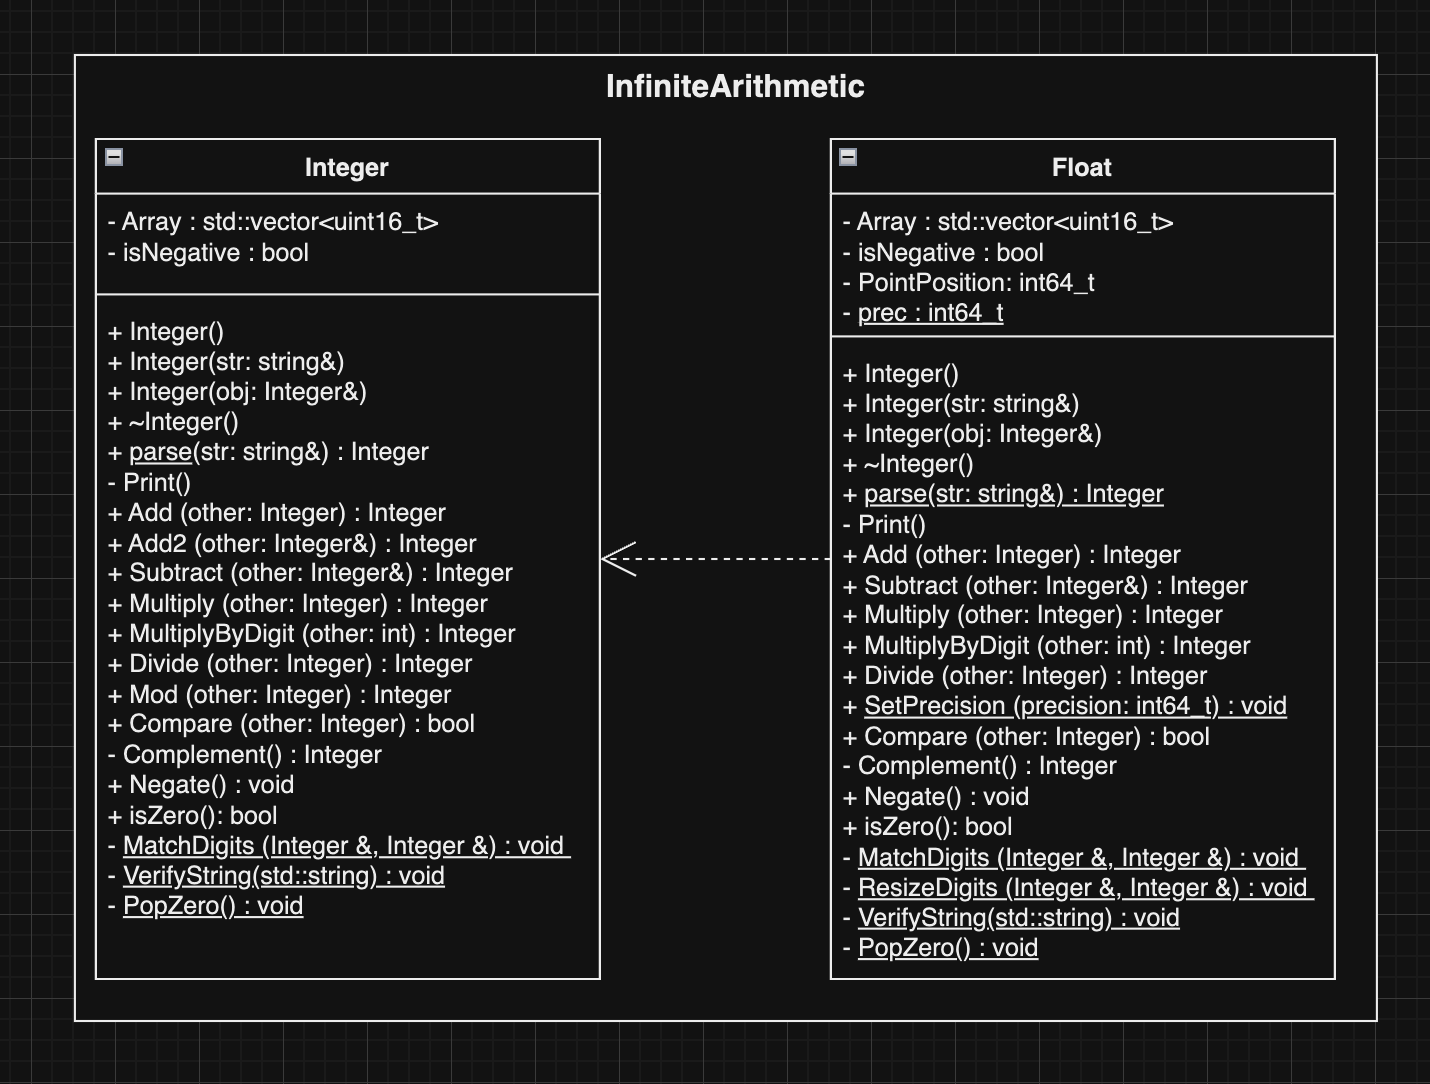
\includegraphics[scale=0.27]{UML Diagram.png}
\end{figure}

